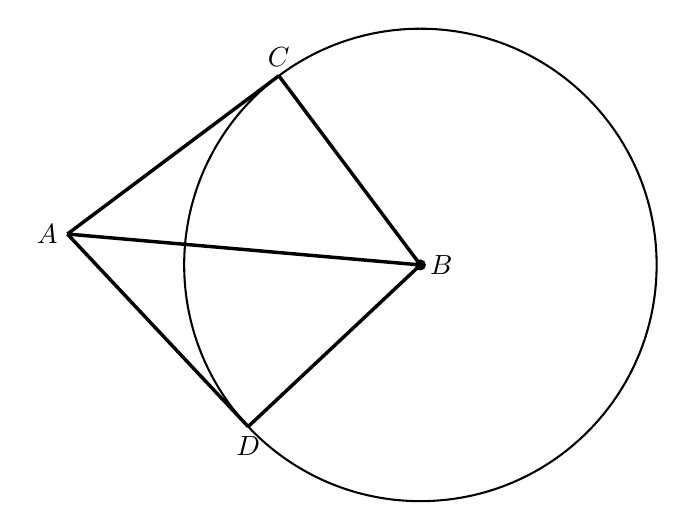
\begin{tikzpicture}[baseline=0]
    % Circle parameters
    \def\r{3} % radius of the circle
    \def\q{4.5} % distance from the center to the external point
    \def\angle{-185} % Rotation angle for the setup

    % x and y coordinates for the tangent points, rotated
    \pgfmathsetmacro{\x}{\r^2/\q} % x coordinate of the point of tangency
    \pgfmathsetmacro{\y}{\r*sqrt(\q^2-\r^2)/\q} % y coordinate of the point of tangency

    % Define points
    \coordinate (O) at (0,0); % Center of the circle
    \coordinate (P) at ({\q*cos(\angle)},{\q*sin(\angle)}); % External point, rotated
    \coordinate (T1) at ({\x*cos(\angle) - \y*sin(\angle)}, {\x*sin(\angle) + \y*cos(\angle)}); % Tangent point 1, rotated
    \coordinate (T2) at ({\x*cos(\angle) + \y*sin(\angle)}, {\x*sin(\angle) - \y*cos(\angle)}); % Tangent point 2, rotated

    % Draw the circle with radius 3
    \draw[line width=.75pt] (0,0) circle (\r);

    % Draw radii and tangent lines
    \draw[line width=1.25pt] (O) -- (T1);
    \draw[line width=1.25pt] (O) -- (T2);
    \draw[line width=1.25pt] (P) -- (T1);
    \draw[line width=1.25pt] (P) -- (T2);
    \draw[line width=1.25pt] (O) -- (P);

    % Mark the center of the circle with a dot
    \fill (O) circle (2pt);
    \node at (O) [right] {$B$};

    % Label the external point and tangent points
    \node at (P) [left] {$A$};
    \node at (T1) [below] {$D$};
    \node at (T2) [above] {$C$};  % Adjusted label for clarity

\end{tikzpicture}